\documentclass[sigplan]{acmart}
\settopmatter{printacmref=false} % Removes citation information below abstract
\renewcommand\footnotetextcopyrightpermission[1]{} % removes footnote with conference information in first column
\usepackage{subcaption}
\usepackage{caption}
\usepackage{array}
\usepackage{multirow}
\usepackage{float}
\usepackage{pdfpages}

\begin{document}

\title{Cloud Infrastructure for DI–FCUL} 

\author{João Oliveira - 56908}
\affiliation{%
 \institution{
  Estudo Orientado \\ 
  Mestrado em Engeharia Informática \\ 
  Faculdade de Ciências, Universidade de Lisboa}
 }
\email{fc56908@alunos.fc.ul.pt}


\begin{abstract}
Cloud computing has become an important tool in academic environments, enabling automation, scalability, and efficient resource utilization. However, many university departments still rely on manually managed virtualized infrastructures, resulting in high administrative overhead, limited flexibility, and inefficient resource allocation.\\

The goal is to design, deploy, and validate a private Infrastructure-as-a-Service (IaaS) cloud for the Department of Informatics of the Faculty of Sciences, University of Lisbon (DI–FCUL or DI),leveraging open-source technologies as Apache Cloudstack as the selected cloud management platform and the Kernel-based Virtual Machine (KVM) as the underlying hypervisor. A key motivation of this project is to replace manual virtual machine provisioning with an automated, self-service infrastructure capable of allocating resources on demand, while preserving institutional control, security, and integration with existing systems.\\

To achieve this, the work is structured into six main phases, following the work plan defined in the project proposal. These phases include an initial requirements analysis and review of the state of the art, the selection and deployment of an access control solution, the design and implementation of the network architecture, the integration of the access control system with the existing Active Directory infrastructure, the deployment and validation of demonstrative prototypes, and the writing of the final dissertation document.\\

The expected outcome is a functional and extensible private cloud IaaS that reduces administrative effort, improves resource utilization, and provides a scalable foundation to support all kinds of learning/research activities at DI–FCUL.
\end{abstract}


\keywords{Cloud Computing, Infrastructure as a Service (IaaS), Apache CloudStack, Virtualization, Academic Cloud}

\pagestyle{plain} % removes running headers

\maketitle
\section{Introduction} \label{sec:introduction}

    Over the past years, cloud computing has transformed the way computing infrastructures are designed and operated, promoting automation, scalability, and flexible resource allocation. These advances have also reached academic environments, where institutions are increasingly adopting the use of private cloud infrastructures to support teaching, research, and administrative workloads through virtualization and automation \cite{alvesUsingCloudBuild2014, bonnerUsingOpenStackImprove2013, oleksiukComparativeStudySupport2021, sheelaDeployingOpenStackCloud2017, vijayakumarPrivateCloudInfrastructure2025}.\\
    
    At DI (Departmento de Informática), this transformation is also underway, through the development of a private Infrastructure-as-a-Service (IaaS) cloud leveraging open-source technologies to enhance efficiency, scalability, and integration with existing systems.\\
    
    The current infrastructure requires manual provisioning and configuration of virtual machines, resulting in high administrative overhead and effort, limited scalability, and inefficient resource usage. This lack of automation makes it difficult to respond quickly to academic demands and maintain consistent, secure environments.\\
    
    Automating infrastructure management is crucial to improving operational efficiency and supporting diverse academic workloads. Open-source IaaS frameworks such as Apache CloudStack\cite{IntroductionApacheCloudStack} or OpenStack\cite{openstack_software} have gained attention in academic environments for their stability and ease of deployment, making them suitable candidates for private cloud infrastructures. Later in Section~\ref{sec:proposed}, these options will be analyzed in more detail, considering both existing literature and the specific requirements of this project.\\
    
    The project aims to design, deploy, and validate a private Infrastructure-as-a-Service (IaaS) cloud for the DI–FCUL. The proposed implementation focuses on automating virtual machine provisioning, integrating user authentication through the institutional Active Directory, and defining basic resource management mechanisms such as service offerings and usage quotas to support different user profiles. The overall objective is to establish a functional and reproducible private cloud environment that can be evaluated under academic usage scenarios and serve as a foundation for future extensions.\\
    
    This report is organized as follows. Section~\ref{sec:background} presents the theoretical and technical background related to cloud computing, virtualization, and cloud management platforms. Section~\ref{sec:related} reviews relevant related work on open-source IaaS frameworks and academic cloud deployments. Section~\ref{sec:proposed} describes the proposed solution and methodology, including architectural decisions and implementation strategy. Section~\ref{sec:results} presents the preliminary results obtained from the proof-of-concept deployment. Finally, Section~\ref{sec:conclusions} discusses the planned future work and provides concluding remarks.

\section{Background} \label{sec:background}
    This section establishes the theoretical and technical foundations that support the design and implementation of the private cloud infrastructure developed for DI.\\
    
    It begins by presenting the core principles of cloud computing, including its fundamental characteristics, service, and deployment models. The discussion then narrows to the Infrastructure as a Service (IaaS) model, which provides the basis for resource provisioning and virtualization within this project.\\
    
    Subsequent subsections describe the role of virtualization technologies, focusing on the Kernel-based Virtual Machine (KVM) as the chosen hypervisor, and detail the architecture of Apache CloudStack — the open-source platform selected for orchestrating and managing the DI private cloud.\\
    
    Finally, this chapter examines networking concepts specific to private cloud environments, such as bridge-based segmentation and network isolation within the FCUL infrastructure, and discusses the automation and resource management mechanisms that enable self-service provisioning through both web and command-line interfaces.\\

    \subsection{Cloud Computing Concepts} \label{sec:background.concepts}
        According to \citeauthor{mellNISTDefinitionCloud} \cite{mellNISTDefinitionCloud}, cloud computing is defined as “a model for enabling ubiquitous, convenient, on-demand network access to a shared pool of configurable computing resources…”. \\
        
        Furthermore, \citeauthor{armbrustCloudsBerkeleyView2009}\cite{armbrustCloudsBerkeleyView2009}, highlighted a paradigm shift in how infrastructures are designed and managed, introducing principles such as elasticity, scalability, and pay-as-you-go resource usage, allowing organizations to dynamically allocate resources based on workload demand.
    
        \subsubsection{Essential Characteristics of Cloud Computing}
            \citeauthor{mellNISTDefinitionCloud}\cite{mellNISTDefinitionCloud} identify five essential characteristics that define cloud computing environments. These characteristics collectively distinguish cloud systems from traditional on-premises infrastructures:
    
            \begin{itemize}
                \item \textbf{On-demand self-service} - Allows users to automatically provision computing resources, without requiring human intervention. 
                
                \item \textbf{Broad network access} - Ensures that services are available over standard network mechanisms and accessible through heterogeneous client platforms.
                
                \item \textbf{Resource pooling} - The provider's ability to serve multiple consumers using a shared pool of physical and virtual resources.
                
                \item \textbf{Rapid elasticity} - Enables systems to scale resources up or down automatically in response to changing workloads. 
            
                \item \textbf{measured service} - Allows cloud platforms to monitor, control, and optimize resource usage automatically.
            
            \end{itemize}
            
            These properties provide the operational foundation for cloud computing, supporting elasticity, flexibility, and cost efficiency.
        
        \subsubsection{Cloud Service Models}
            Cloud services are divided into three categories\cite{mellNISTDefinitionCloud}:
            \begin{itemize}
                \item \textit{Infrastructure as a Service (IaaS)} - The user creates and manages virtual machines and storage, controlling the system but not the physical hardware (e.g., Amazon EC2).
            
                \item \textit{Platform as a Service (PaaS)} - The user builds and runs their own applications using tools provided by the cloud provider (e.g., Google App Engine).
            
                \item \textit{Software as a Service (SaaS)} - The user uses ready-to-go applications over the internet, without managing anything technical (e.g., Microsoft 365).
            \end{itemize}
        
        \subsubsection{Cloud Deployment Models}
            Cloud infrastructures can be deployed under different models depending on ownership, access control, and purpose. There are four main deployment models\cite{mellNISTDefinitionCloud}:
            \begin{itemize}
                \item \textit{Public clouds} - Owned and operated by third-party providers and available to multiple users.
                \item \textit{Private clouds} - Dedicated to a single organization, offering higher control and security. This is the model adopted for this project.
                \item \textit{Community clouds} - Shared among organizations with common goals or compliance requirements.
                \item \textit{Hybrid clouds} - Which combine two or more models to balance flexibility, scalability, and governance. 
            \end{itemize}
            
        In the context of this project, the most relevant aspect is the IaaS model and the Private cloud deployment model, since it aligns with the expected structure to develop. This will be explored in more detail in Subsection ~\ref{sec:background.iaas}.

    \subsection{Infrastructure as a Service (IaaS)} \label{sec:background.iaas}
    
        \subsubsection{Definition and Core Components}
            Infrastructure as a Service (IaaS) constitutes the foundational layer of the cloud computing stack, providing users with access to virtualized computing resources such as processing, storage, and networking through APIs or graphical interfaces \cite{mellNISTDefinitionCloud}. In this model, the cloud provider manages the physical infrastructure, while consumers retain control over the operating systems, middle-ware, and applications they deploy. Compared to Platform as a Service (PaaS) and Software as a Service (SaaS), IaaS offers the lowest level of abstraction, giving users greater flexibility and configurability at the cost of higher administrative responsibility.\\
            
            A typical IaaS architecture is composed of several key components:
            \begin{itemize}
                \item \textit{Compute layer} - Hosts and manages virtual machines through hypervisors;
                \item \textit{Storage layer} - Provides persistent volumes and snapshot mechanisms;
                \item \textit{Network layer} - Abstracts connectivity and security through virtualized switches and firewalls;
            \end{itemize}
            
            These resources are orchestrated by a management layer that automates provisioning, scaling, and monitoring, typically through centralized controllers and user-facing portals. Open-source frameworks such as \textit{OpenStack} or \cite{openstack_software}, \textit{Apache CloudStack} \cite{IntroductionApacheCloudStack} implement these mechanisms, offering modular platforms for infrastructure automation and orchestration.\\
            
            The implementation of IaaS relies fundamentally on virtualization, which enables the abstraction and efficient allocation of hardware resources. The following subsection explores the principles of virtualization and hypervisors, focusing on the Kernel-based Virtual Machine (KVM) as the chosen technology for the DI private cloud.
            
            \subsubsection{Advantages and Challenges of IaaS}
                The main advantages of the IaaS model include scalability, resource isolation, and cost efficiency, achieved through dynamic allocation and on-demand provisioning of resources \cite{armbrustCloudsBerkeleyView2009}. However, it also introduces challenges related to multi-tenancy, network security, and effective resource scheduling.
            
            \subsubsection{IaaS in Academic Environments}
                In academic environments, where infrastructure must accommodate diverse research and teaching workloads, IaaS provides a flexible foundation that allows departments to autonomously deploy and manage computing environments. Previous studies have shown that adopting private IaaS solutions in universities enhances system availability, reduces hardware costs, and simplifies resource management \cite{alvesUsingCloudBuild2014,bonnerUsingOpenStackImprove2013,oleksiukExperienceMaintenanceAcademic2021}.

            \subsubsection{Summary}    
                For the DI-FCUL, the IaaS model offers a technical and organizational advantage by integrating virtualization, authentication, and automation into a unified private cloud. This approach allows academic users to request, configure, and manage virtual machines through self-service portals, improving efficiency while maintaining centralized control and compliance with institutional policies.


    \subsection{Virtualization and Hypervisors} \label{sec:background.virtualization}
        Virtualization plays a fundamental role in enabling cloud computing by allowing physical hardware resources to be abstracted into isolated virtual environments. \\
        
        Through this, multiple operating systems and applications can run concurrently on a single host while sharing underlying compute, storage, and networking resources. \cite{IBMVirtualization, ratnanginirekComparativeStudyHypervisor2021}
        This abstraction layer is managed by a hypervisor, which allocates and controls access to these resources, ensuring performance isolation and efficient utilization.\\ 
        
        This section introduces the core concepts of virtualization and examines the different types of hypervisors, with particular emphasis on the Kernel-based Virtual Machine (KVM) due to its relevance in open-source IaaS frameworks such as Apache CloudStack.
        
        \subsubsection{Concept of Virtualization}
            Virtualization, a concept that dates back to the 1960s\cite{ratnanginirekComparativeStudyHypervisor2021, IBMVirtualization}, creates an abstraction layer over computer hardware, the system physical components into multiple virtual machines (VMs) with their own operating system (OS) and behaves like a separate physical computer, despite sharing the same underlying hardware \cite{IBMVirtualization}.\\

            Today, virtualization forms the foundation of cloud computing by allowing providers to dynamically allocate and manage resources, supporting the scalability and elasticity required by IaaS environments \cite{IBMVirtualization}.
        
        \subsubsection{Types of Hypervisors}
            Running an operating system (OS) within another OS is made possible by virtualization, specifically through the use of hypervisors. 
            The physical hardware that hosts the hypervisor is referred to as the \textit{host}, while the VMs that utilize its resources are called \textit{guests} \cite{RedhatKVM}. 
            Hypervisors manage the hardware resources of the host machine (CPU, Memory, etc...)and allocate them to the guest systems, ensuring efficient and secure execution of applications \cite{ratnanginirekComparativeStudyHypervisor2021}. \\
            
            To perform these tasks, hypervisors rely on several operating system–level components, including a memory manager, process scheduler, input/output (I/O) stack, device drivers, security manager and network stack, which together enable the creation and operation of virtual environments.\\
            
            There are two categories of hypervisors \cite{IBMVirtualization}:
            \begin{itemize}
                \item \textbf{Type~1 (bare-metal)} hypervisors interact directly with the physical hardware, effectively replacing a traditional operating system. 
            They are most commonly used in server and data center environments, where a single physical server is partitioned into multiple isolated segments, each capable of running its own OS and applications.
            
                \item \textbf{Type~2 (hosted)} hypervisors, on the other hand, run as software applications on top of an existing operating system. 
            These are typically deployed on endpoint or desktop systems to run additional guest OSs for testing and development purposes. 
            Because they depend on the host OS to access and coordinate underlying hardware resources, Type~2 hypervisors inherently introduce additional overhead and reduced performance.
            \end{itemize}
    
            Among Type~1 hypervisors, the Kernel-based Virtual Machine (KVM) has gained prominence as an open-source solution that integrates directly with the Linux kernel \cite{kivityKvmLinuxVirtual}, providing near-native performance \cite{algarniPerformanceEvaluationXen2018} and full compatibility with modern cloud orchestration platforms such as Apache CloudStack and OpenStack \cite{vijayakumarPrivateCloudInfrastructure2025}.

        \subsubsection{Kernel-based Virtual Machine (KVM)} \label{sec:background.virtualization.kvm}
            Kernel-based Virtual Machine (KVM) is an open-source virtualization technology integrated into the Linux kernel that enables Linux to operate as a Type~1 hypervisor, supporting the creation and execution of virtual machines (VMs)~\cite{kivityKvmLinuxVirtual2007, RedhatKVM}. In KVM-based deployments, each VM is implemented as a regular Linux process, allowing it to benefit from the kernel’s scheduling, memory management, and security mechanisms, which contributes to strong isolation and near-native performance~\cite{kivityKvmLinuxVirtual2007}.\\
            
            In this project, KVM is used as the underlying hypervisor because it integrates naturally with Linux-based server environments and is widely supported by open-source IaaS platforms. CloudStack interacts with KVM through \textit{libvirt}, which provides a standardized interface for VM lifecycle operations and resource control~\cite{vijayakumarPrivateCloudInfrastructure2025}. This combination enables consistent automation of provisioning and management tasks, aligning with the project's goal of deploying a maintainable private IaaS infrastructure for DI-FCUL.
    
    \subsection{Apache CloudStack} \label{sec:background.cloudstack}
    	Apache CloudStack is an open-source IaaS platform designed to manage and orchestrate compute, storage, and networking resources for the deployment of a private and public cloud infrastructures~\cite{IntroductionApacheCloudStack}. Its architecture emphasizes simplicity, robustness, and operational predictability, which has contributed to its adoption in private and academic cloud environments~\cite{lynnComparativeStudyCurrent2015}.\\
    
    	CloudStack supports multiple hypervisors, including KVM, XenServer, and Hyper-V\cite{IntroductionApacheCloudStack}, although KVM is the most commonly used in open-source deployments due to its performance and native integration with Linux~\cite{IntroductionApacheCloudStack, algarniPerformanceEvaluationXen2018, vijayakumarPrivateCloudInfrastructure2025}. For these reasons, KVM was selected as the hypervisor for this project, as discussed in Section~\ref{sec:background.virtualization.kvm}.
    
    	\subsubsection{Architecture Overview}
    		CloudStack follows a modular architecture centered around a \textbf{Management Server}, which acts as the control plane of the cloud environment. The Management Server provides a web-based interface and a programmatic API, and is responsible for orchestrating the lifecycle of virtual machines and associated resources, enforcing access control policies, and coordinating interactions with underlying infrastructure components~\cite{IntroductionApacheCloudStack}.\\
    
    		Compute hosts run a lightweight \textbf{CloudStack Agent}, which executes commands issued by the Management Server and interacts with the hypervisor through \textit{libvirt}. This design centralizes management logic while distributing execution across the compute infrastructure.
    
    	\subsubsection{Resource Organization Model}
    		CloudStack organizes infrastructure resources hierarchically to support scalability and simplified management. In the context of this project, the most relevant elements of this hierarchy are:
    
            \begin{itemize}
                \item \textbf{Zone}, representing a logical datacenter boundary;
                \item \textbf{Cluster}, grouping hosts with similar configurations and shared primary storage;
                \item \textbf{Host}, corresponding to an individual compute server running the hypervisor.
            \end{itemize}
    
    		This model provides clear scheduling and isolation domains while remaining suitable for both small-scale and larger private cloud deployments\cite{vogelPrivateIaaSClouds2016}.
    
    	\subsubsection{Compute and Storage Management}
    		CloudStack manages the full lifecycle of virtual machines, including provisioning, monitoring, and retirement. Virtual machines are instantiated based on predefined service offerings and templates, with placement decisions handled by the Management Server according to resource availability and policy constraints.\\
    
    		From a storage perspective, CloudStack distinguishes between \textit{primary storage}, which hosts virtual machine disk volumes, and \textit{secondary storage}, which stores templates, ISO images, and snapshots. This separation simplifies VM lifecycle operations and supports efficient reuse of images across the cloud environment~\cite{IntroductionApacheCloudStack}.\\
    
            Overall, Apache CloudStack provides a flexible and extensible platform for managing private IaaS infrastructures. Its architecture and resource model form the basis for the deployment described in the following sections.
    
    	\subsubsection{Automation and Interfaces}
    		CloudStack provides multiple interfaces that support both interactive management and full automation of cloud operations. A web-based graphical interface allows administrators and users to deploy and manage virtual machines and associated resources, while a REST-like API exposes all management functions for programmatic access~\cite{IntroductionApacheCloudStack}.\\
    
    		For command-line interaction and automation, CloudStack offers \textit{CloudMonkey}, a lightweight CLI that acts as a convenient wrapper around the API and supports both interactive and scripted usage~\cite{CloudStackCloudmonkeyCLI}. Together, these interfaces enable self-service provisioning and integration with institutional management workflows.
    
    	\subsubsection{Summary}
                Apache CloudStack offers a comprehensive and modular architecture for orchestrating virtualized resources in private cloud environments. Its hierarchical model, built-in networking and storage services, hypervisor-agnostic design, and automation interfaces make it particularly suitable for academic institutions. These capabilities form the basis for the implementation of the DI-FCUL private cloud, described in later sections.

    \subsection{Networking in Private Cloud Environments} \label{sec:background.networking}
        Networking is a critical component of any cloud infrastructure, as it enables communication between virtual machines, hypervisor hosts, storage systems, and the cloud management plane. In Infrastructure as a Service (IaaS) environments, physical networking is augmented and frequently abstracted by virtual networking constructs that provide flexibility, isolation, and scalability. These mechanisms are particularly relevant in KVM-based deployments, where virtual switches and bridges form the foundation of network.
        
        \subsubsection{Virtual Networks and Linux Bridges}
            Virtual networking in Linux-based hypervisors relies on the use of \textit{Linux bridges}, which behaves like a network switch within the kernel \cite{liuIntroductionLinuxInterfaces2018}. According to the official Linux Kernel Networking Documentation, a bridge forwards and filters Ethernet frames between physical and virtual interfaces, effectively emulating the behaviour of a physical switch~\cite{linuxbridgeDocs}.\\

            In KVM, each virtual machine is associated with a \textit{TAP interface}—a virtual Ethernet device that represents the VM’s network card. These TAP interfaces are attached to a Linux bridge such as \texttt{br0} or \texttt{cloudbr0}. The bridge may be connected to a physical NIC, enabling VMs to participate directly in the physical network, or to other virtual networks depending on the cloud configuration. The KVM Networking Documentation describes this model as the standard method for integrating VMs into the host’s Layer-2 network domain~\cite{kvmNetworkingDocs}.\\

            Libvirt, which abstracts virtualization management for hypervisors including KVM, provides a higher-level interface for defining and controlling virtual networks. It supports multiple topologies—bridge, routed, isolated, and NAT networks—and uses Linux networking primitives (bridges, iptables, dnsmasq) to configure DHCP, DNS, firewalling, and packet forwarding~\cite{libvirtNetworking}. Cloud orchestration platforms such as Apache CloudStack rely on libvirt to control VM network interfaces in a consistent and portable manner.
            
            \begin{figure}[H]
                \centering
                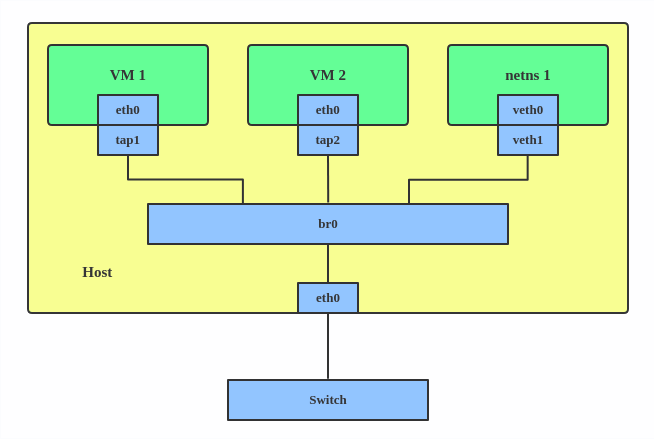
\includegraphics[width=1\linewidth]{photos/bridge.png}
                \caption{Linux bridge example}
                \label{fig:placeholder}
            \end{figure}

\section{Related Work} \label{sec:related}
    \subsection{Open-Source IaaS Frameworks}
        This section reviews previous works related to the fields being studied, namely open-source Infrastructure as a Service (IaaS) frameworks, virtualization technologies and hypervisors, CloudStack deployments in academic environments, as well as resource management and automation strategies in private clouds. 
        The objective is to provide an overview of the current state of the art in these domains, identifying key technological approaches, design choices, and research trends that inform the development of this project. 
        By analyzing these studies, it becomes possible to highlight the advantages and limitations of existing solutions and to justify the architectural and technological decisions adopted for the implementation of a private CloudStack-based infrastructure at DI.\\
    
        Several open-source IaaS platforms have emerged as alternatives to commercial cloud solutions, motivated by the need to avoid vendor lock-in, maintain institutional autonomy, enable cost-effective private cloud deployments, and provide greater flexibility for customization~\cite{lynnComparativeStudyCurrent2015}. Among these, \textbf{OpenStack}, \textbf{Apache CloudStack}, and \textbf{OpenNebula} have consistently appeared as the most prominent frameworks, while \textbf{Eucalyptus} and \textbf{Nimbus} are referenced primarily for more specialized contexts~\cite{lynnComparativeStudyCurrent2015, arunaOpenSourceIaaS2016}. In 2014, OpenStack was reported as the most popular platform, followed by CloudStack and OpenNebula\cite{williamsTopOpenSource2014}. This trend remains reflected in the literature, where OpenStack and CloudStack are the most frequently analyzed and deployed IaaS platforms across academic and organizational settings.
    
        \subsubsection{Architectural and Design Differences}
            Comparative analyses of open-source IaaS platforms consistently highlight fundamental architectural differences among the main frameworks: OpenStack, Apache CloudStack, OpenNebula, Eucalyptus, and Nimbus. A recurring theme in the literature concerns the contrast between highly modular platforms and those following more integrated or lightweight designs. \textbf{OpenStack} adopts a distributed, service-oriented architecture in which each subsystem is deployed as an independent service with well-defined APIs. This supports extensibility and large-scale customization but introduces notable deployment and operational complexity due to the decentralized design, sheer number of components and the different configuration possibilities~\cite{barkatOpenSourceSolutions2015}. In contrast, \textbf{Apache CloudStack} follows a more integrated, monolithic architecture centered around a single Management Server, resulting in a cohesive control plane with fewer moving parts and a simpler installation and upgrade workflow. \textbf{OpenNebula} offers a lightweight centralized design that typically requires only a single management frontend, thereby reducing administrative overhead at the cost of reduced extensibility~\cite{arunaOpenSourceIaaS2016}. Eucalyptus and Nimbus adopt more specialized design goals, particularly with regard to AWS API compatibility and scientific computing.
        
        \subsubsection{Deployment and Operational Complexity}
            These architectural distinctions translate directly into differences in deployment and operational behavior. Across comparative studies, \textbf{OpenStack} is consistently identified as the most demanding platform to deploy and maintain, with its modular architecture requiring substantial system administration expertise and extensive configuration~\cite{lynnComparativeStudyCurrent2015, barkatOpenSourceSolutions2015}. By contrast, \textbf{CloudStack}'s integrated controller and unified workflows make it more straightforward to install and operate, reducing the likelihood of configuration inconsistencies and making it attractive for private cloud environments with limited operational teams. \textbf{OpenNebula} is frequently cited as the easiest platform to deploy and manage due to its minimal footprint, positioning it as a suitable solution for smaller academic laboratories or lightweight research infrastructures~\cite{barkatOpenSourceSolutions2015}. Experimental evaluations further reinforce these tendencies: OpenStack and CloudStack both support a broad set of storage, hypervisor, and network technologies, contributing to stronger resiliency characteristics, with OpenStack achieving the highest feature coverage and CloudStack following closely~\cite{vogelPrivateIaaSClouds2016}. OpenNebula, while simpler, provides more limited support in these dimensions, aligning with its streamlined design.
        
        \subsubsection{Experimental Behaviour and Performance Evaluation}
            \citeauthor{vogelPrivateIaaSClouds2016}\cite{vogelPrivateIaaSClouds2016} compares OpenStack, CloudStack and OpenNebula under identical KVM-based conditions and report that all three systems exhibit broadly similar behaviour under moderate workloads, although with consistent differences in stability and execution times. Their results show that \textbf{OpenStack} achieves the best overall performance and the lowest variance across repeated operations, followed closely by \textbf{CloudStack}, while \textbf{OpenNebula} performs less favourably, particularly in storage and networking tasks. Complementing these findings, \citeauthor{paradowskiBenchmarkingPerformanceOpenStack2014}\cite{paradowskiBenchmarkingPerformanceOpenStack2014} also observe that \textbf{OpenStack} outperforms CloudStack in several metrics. They suggest that these differences may be influenced by implementation, as OpenStack is written primarily in Python while CloudStack is Java-based. Although the absolute performance gaps are not large enough to be decisive in isolation, the combined evidence indicates that OpenStack tends to provide the most stable and efficient performance profile, with CloudStack performing closely.
        
        \subsubsection{Summary}
            Across qualitative, experimental, and performance-based studies, a consistent consensus emerges: \textbf{OpenStack} and \textbf{CloudStack} are the two most mature and widely adopted open-source IaaS frameworks, each occupying distinct roles. OpenStack excels in flexibility, ecosystem breadth, and overall performance, but requires substantial expertise and operational effort to deploy and maintain effectively. By contrast, CloudStack provides a more integrated and administratively manageable solution, making it particularly suitable for private cloud environments where simplicity, predictability, and operational stability are prioritized. Other open-source platforms present specific strengths within narrower domains, but OpenStack and CloudStack remain the most complete and robust solutions currently available.

    \subsection{IaaS Deployments in Academic and Research Environments} \label{sec:related.academicclouds}

        Academic institutions increasingly adopt private cloud infrastructures to address pedagogical, operational, and economic needs. Universities require flexible and centrally managed computing environments to support teaching laboratories, research workloads, and project-based learning, while retaining institutional control over data, identity systems, and security policies~\cite{lynnComparativeStudyCurrent2015, vijayakumarPrivateCloudInfrastructure2025}. Private clouds provide this flexibility by enabling on-demand provisioning of virtual machines, reducing dependence on physical computer rooms and simplifying maintenance workflows for IT teams. Studies such as \citeauthor{alvesUsingCloudBuild2014}\cite{alvesUsingCloudBuild2014} and \citeauthor{bonnerUsingOpenStackImprove2013}\cite{bonnerUsingOpenStackImprove2013} show that virtualised laboratory environments improve reproducibility, resource utilisation, and student accessibility, particularly when remote access or rapidly reconfigurable setups are required.\\
        
        Operational and financial considerations further motivate the adoption of open-source IaaS platforms in academia. The elasticity of private clouds allows institutions to accommodate highly variable workloads driven by academic calendars and research activities~\cite{sheelaDeployingOpenStackCloud2017}. At the same time, open-source solutions reduce licensing costs and allow existing hardware to be repurposed, avoiding the financial unpredictability associated with commercial pay-per-use cloud services~\cite{vijayakumarPrivateCloudInfrastructure2025, alvesUsingCloudBuild2014}. Moreover, the ability to integrate with institutional authentication systems and enforce customised usage policies makes open-source IaaS frameworks particularly suited to environments seeking autonomy and robust administrative control~\cite{oleksiukExperienceMaintenanceAcademic2021}.\\

        Overall, the literature consistently shows that private academic clouds provide a scalable, cost-efficient, and institutionally controlled solution for supporting modern educational and research activities.
        
        \subsubsection{Motivations for Academic and Institutional Clouds}
            The adoption of private cloud infrastructures in academic environments is driven by a combination of pedagogical, operational, and economic needs. Universities increasingly require flexible, scalable, and centrally managed computing environments to support teaching laboratories, research workloads, and project-based learning, while retaining institutional control over data, identity systems, and security policies. A key motivation is the virtualization of teaching laboratories: traditional physical labs demand extensive software installation and maintenance efforts from IT teams, which must prepare machines in advance for each course or semester. Cloud-based virtual labs significantly reduce this burden by enabling pre-configured environments to be provisioned on demand, improving resource utilization \cite{bonnerUsingOpenStackImprove2013, alvesUsingCloudBuild2014}. These environments also enhance reproducibility and flexibility, allowing students to deploy isolated virtual machines for practical coursework without depending on fixed physical facilities.\\
            
            University workloads fluctuate considerably throughout the academic year due to coursework deadlines, laboratory-intensive modules, research cycles, and short-term training programs. Private cloud infrastructures allow institutions to allocate and reclaim compute resources dynamically, mitigating the administrative overhead associated with managing heterogeneous physical servers~\cite{sheelaDeployingOpenStackCloud2017}. Economic considerations also contribute to this trend: open-source IaaS platforms reduce licensing costs and enable institutions use resources more efficiently, offering a predictable and financially sustainable alternative to commercial public clouds, whose pay-per-use pricing introduces budget variability that is often incompatible with academic planning~\cite{vijayakumarPrivateCloudInfrastructure2025, alvesUsingCloudBuild2014, bonnerUsingOpenStackImprove2013}. Moreover, open-source cloud platforms allow universities to integrate with existing campus authentication systems and define customized access, quota, and security policies, thereby preserving autonomy and tailoring the infrastructure to institutional requirements~\cite{lynnComparativeStudyCurrent2015, oleksiukExperienceMaintenanceAcademic2021}.\\
            
            In the context of DI, these motivations are particularly significant. They manage multiple teaching laboratories and supports a diverse set of computational requirements across courses and research groups, creating substantial operational overhead when relying on traditional physical infrastructures. A private, open-source IaaS platform can reduce this burden through automated provisioning and centralized management, while enabling the reuse of existing hardware and avoiding the fluctuating costs associated with commercial public cloud services. These factors align directly with the requirements of the planned CloudStack-based deployment at DI.
        
        \subsubsection{Experiences Using OpenStack in Academic Clouds}
            OpenStack has been widely explored in academic environments to support virtualized teaching laboratories. \citeauthor{bonnerUsingOpenStackImprove2013}\cite{bonnerUsingOpenStackImprove2013} describe the deployment of an private cloud to enhance the student experience in Huddersfield University, enhancing the students learning experience. Their study reports improvements in reproducibility, flexibility, and remote accessibility, particularly in modules requiring rapidly reconfigurable computational environments. Also they report operational savings resulting from reduced effort in preparing hardware, software, and dedicated laboratory space. \citeauthor{sheelaDeployingOpenStackCloud2017}\cite{sheelaDeployingOpenStackCloud2017} describe the step-by-step deployment of OpenStack in a university environment, noting that its multi-service architecture requires substantial setup and coordination between components.\\

            Overall, the literature shows that OpenStack offers powerful self-service capabilities, strong support for multi-tenant virtualization, and effective resource elasticity, making it well suited to pedagogical and research-driven use cases. However, its deployment and maintenance demands could represent a significant barrier for many academic environments, particularly those operating with small or moderately staffed system administration teams.           
        
        \subsubsection{Experiences Using CloudStack in Academic Clouds}
            Several studies report the use of CloudStack in environments where operational simplicity and predictable behavior are prioritized, in part by its well-structured and user-oriented graphical interface, which lowers the entry barrier for those who interact with it.~\cite{lynnComparativeStudyCurrent2015, oleksiukComparativeStudySupport2021}. The availability of a dedicated user portal allows end users to provision and manage virtual machines in a self-service manner, supporting common academic use cases such as teaching laboratories and project-based coursework while reducing direct intervention from administrators.\\
            
            From an operational perspective, CloudStack deployments in this contexts show sufficient stability to support a wide range of activities, from introductory IT training to more advanced experimentation in cloud computing.~\cite{oleksiukComparativeStudySupport2021, vijayakumarPrivateCloudInfrastructure2025}. The platform’s networking capabilities, including support for isolated networks and firewall integration, are highlighted as particularly valuable for separating workloads and ensuring data integrity across distinct courses or research projects. While some isolated issues have been documented, these are typically associated with underlying infrastructure configuration rather than inherent platform limitations.\\
            
            A recurring theme across the analyzed studies is it's the suitability for institutions operating with limited hardware resources and small system administration teams. Compared to more highly modular platforms, CloudStack is consistently characterized as having a moderate installation complexity and a more manageable operation, making it more accessible to environments without extensive cloud expertise.~\cite{vogelPrivateIaaSClouds2016, oleksiukExperienceMaintenanceAcademic2021}. The availability of comprehensive APIs further enables the automation of repetitive administrative tasks, allowing institutions to scale their infrastructure incrementally as demand grows without requiring significant reconfiguration or downtime.~\cite{vijayakumarPrivateCloudInfrastructure2025}.
        
        \subsubsection{Comparative Insights and Requirements of Academic Clouds}
            Based on the reviewed literature, a consistent set of high-level requirements emerges for private cloud infrastructures deployed in academic environments. One of the primary concerns is \textit{economic sustainability and resource optimization}, as academic institutions typically operate under thigh budgets and hardware availability, which minimizes operational and maintenance costs while maximizing existing resources usage~\cite{lynnComparativeStudyCurrent2015, alvesUsingCloudBuild2014, vijayakumarPrivateCloudInfrastructure2025}. Open-source IaaS platforms are therefore favored, as they reduce licensing costs and allow institutions to retain full control over their infrastructure.\\

            Another requirement pointed out is \textit{ease of use and pedagogical accessibility}. The interface must be simple and there should be a level of automation, to save time and effort to focus on other activities rather than on infrastructure management~\cite{bonnerUsingOpenStackImprove2013, oleksiukExperienceMaintenanceAcademic2021}. This is particularly relevant in teaching laboratories, where rapid provisioning and reconfiguration of environments are frequent requirements.\\

            \textit{Scalability and elasticity} are also essential characteristics of academic clouds. Workloads tend to fluctuate significantly throughout the academic year, with peaks and troughs during the year~\cite{sheelaDeployingOpenStackCloud2017}, therefore, dynamic allocation and reclamation of resources without excessive administrative effort are highly desirable. In parallel, \textit{flexibility and customization} are required, often demanding non-standard configurations and direct access to virtualized resources~\cite{vijayakumarPrivateCloudInfrastructure2025}.\\

            Finally, \textit{service continuity and data integrity} are fundamental to ensure reliable operation through effective user isolation, network segmentation, and backup mechanisms, avoiding possible data loss or service disruption~\cite{oleksiukExperienceMaintenanceAcademic2021}.\\
            
            When these requirements are considered, the limitations of highly modular platforms such as OpenStack become evident for small or moderately staffed administrative teams. Although OpenStack offers extensive functionality and broad technological support, its architecture introduces significant deployment and operational complexity, requiring specialized expertise and sustained administrative effort~\cite{lynnComparativeStudyCurrent2015, barkatOpenSourceSolutions2015}. In contrast, CloudStack adopts a more efficient design, with its integrated architecture and simplified orchestration model, which reduces configuration overhead and supports day-to-day operations through a graphical interface and automation mechanisms~\cite{vogelPrivateIaaSClouds2016, oleksiukExperienceMaintenanceAcademic2021}. OpenNebula cloud also be a good alternative, as it follows a lightweight and centralized approach based on standard Linux services, resulting in a reduced operational footprint and a gentler learning curve for Unix-oriented administrative teams~\cite{oleksiukComparativeStudySupport2021}.\\

            Overall, the literature indicates that while OpenStack offers unmatched flexibility and ecosystem breadth, CloudStack effectively satisfy the practical requirements of academic private clouds operated by small teams. Among these, CloudStack is often identified as offering the most balanced trade-off between robustness, flexibility, and administrative simplicity, making it particularly well suited for institutional deployments such as the one proposed for DI-FCUL.
        
        \subsubsection{Summary and Relevance to DI-FCUL}\label{sec:related.summary}.
            The literature highlights a consistent set of requirements including operational simplicity, predictable behavior, efficient use of limited hardware resources, and the ability to integrate with existing institutional systems. Studies further emphasize the importance of reducing administrative overhead, particularly in contexts where system administration teams are small and infrastructure budgets are constrained.\\

            CloudStack emerges as a suitable solution due to its integrated architecture, unified management model, and emphasis on operational stability and simplicity, which directly addresses many of the challenges identified. Compared to highly modular platforms such as OpenStack, CloudStack offers a more accessible deployment and maintenance process, while still providing sufficient flexibility and scalability.\\
            
            These characteristics align with the objectives described in the project proposal. The proposed solution emphasizes centralized management, controlled resource provisioning, and compatibility with existing institutional infrastructures. Within this scope, the literature supports the selection of CloudStack as a suitable technological foundation, providing the necessary balance between functionality, manageability, deployment simplicity and institutional control.

\section{Proposed Solution and Methodology} \label{sec:proposed}
    \subsection{Problem Definition and Objectives}
        As said in the previously, section~\ref{sec:introduction}, the current infrastructure at the DI requires heavy manual VM management, leading to increased administrative effort, limited scalability, and reduced flexibility supporting academic workloads.\\

        The main objective of this project is to design and deploy a IaaS cloud that automates provisioning and management of virtualized resources (storage, compute and network) within the DI environment. The proposed solution aims to provide controlled self-service access to virtual machines for different user profiles, integrate with the existing institutional authentication infrastructure, and maintain centralized governance over compute, storage, and networking resources. The scope of this work is limited to a private cloud deployment, accessible within the FCUL's network and does not include large-scale geographically distributed scenarios.\\


    \subsection{Requirements Analysis}
        This section presents the main requirements identified for the design and deployment of the desired private cloud infrastructure. These requirements were derived from the analysis of the existing infrastructure, the review of related work, practical constraints associated with this type of system and the requested and the project objectives. They are divided into functional and non-functional requirements.
    
        \subsubsection{Functional Requirements}
            The proposed cloud infrastructure must support the following functional requirements:
            
            \begin{itemize}
                \item The system must allow the creation, deployment, and management of virtual machines through a centralized cloud platform, including command-line and API-based interactions.
                \item The platform must integrate with the existing Active Directory infrastructure, enabling centralized authentication and role-based access control.
                \item Authorized users should be able to request and manage virtual machines through a web-based interface or programmatic APIs, according to their assigned roles.
                \item Compute, storage, and networking resources must be defined at the cloud management level and allocated dynamically to virtual machines during deployment.
                \item The system must support the definition and enforcement of quotas and service offerings to regulate resource usage (e.g., compute, memory, and storage) among different user profiles.
            \end{itemize}
        
        \subsubsection{Non-Functional Requirements}
            In addition to functional capabilities, the infrastructure must satisfy several non-functional requirements:
    
            \begin{itemize}
                \item The solution must be compatible with the current infrastructure, minimizing disruption to existing services. This includes the Institution Network and Authentication System.
                \item The platform should be manageable without too much effort, with predictable behavior and low operational overhead.
                \item The architecture must support incremental expansion as demand increases.
                \item The system should provide stable operation suitable for continuous academic use.
                \item Access to resources must be controlled and traceable, ensuring isolation between users and compliance with institutional policies.
            \end{itemize}

    \subsection{Architectural Overview}
        The proposed infrastructure is going to be deployed within the premises of DI–FCUL. The architecture follows a centralized management model, in which orchestration and control are handled by a dedicated management server, while execution is distributed across a set of virtualization hosts.\\

        \begin{figure}[H]
            \centering
                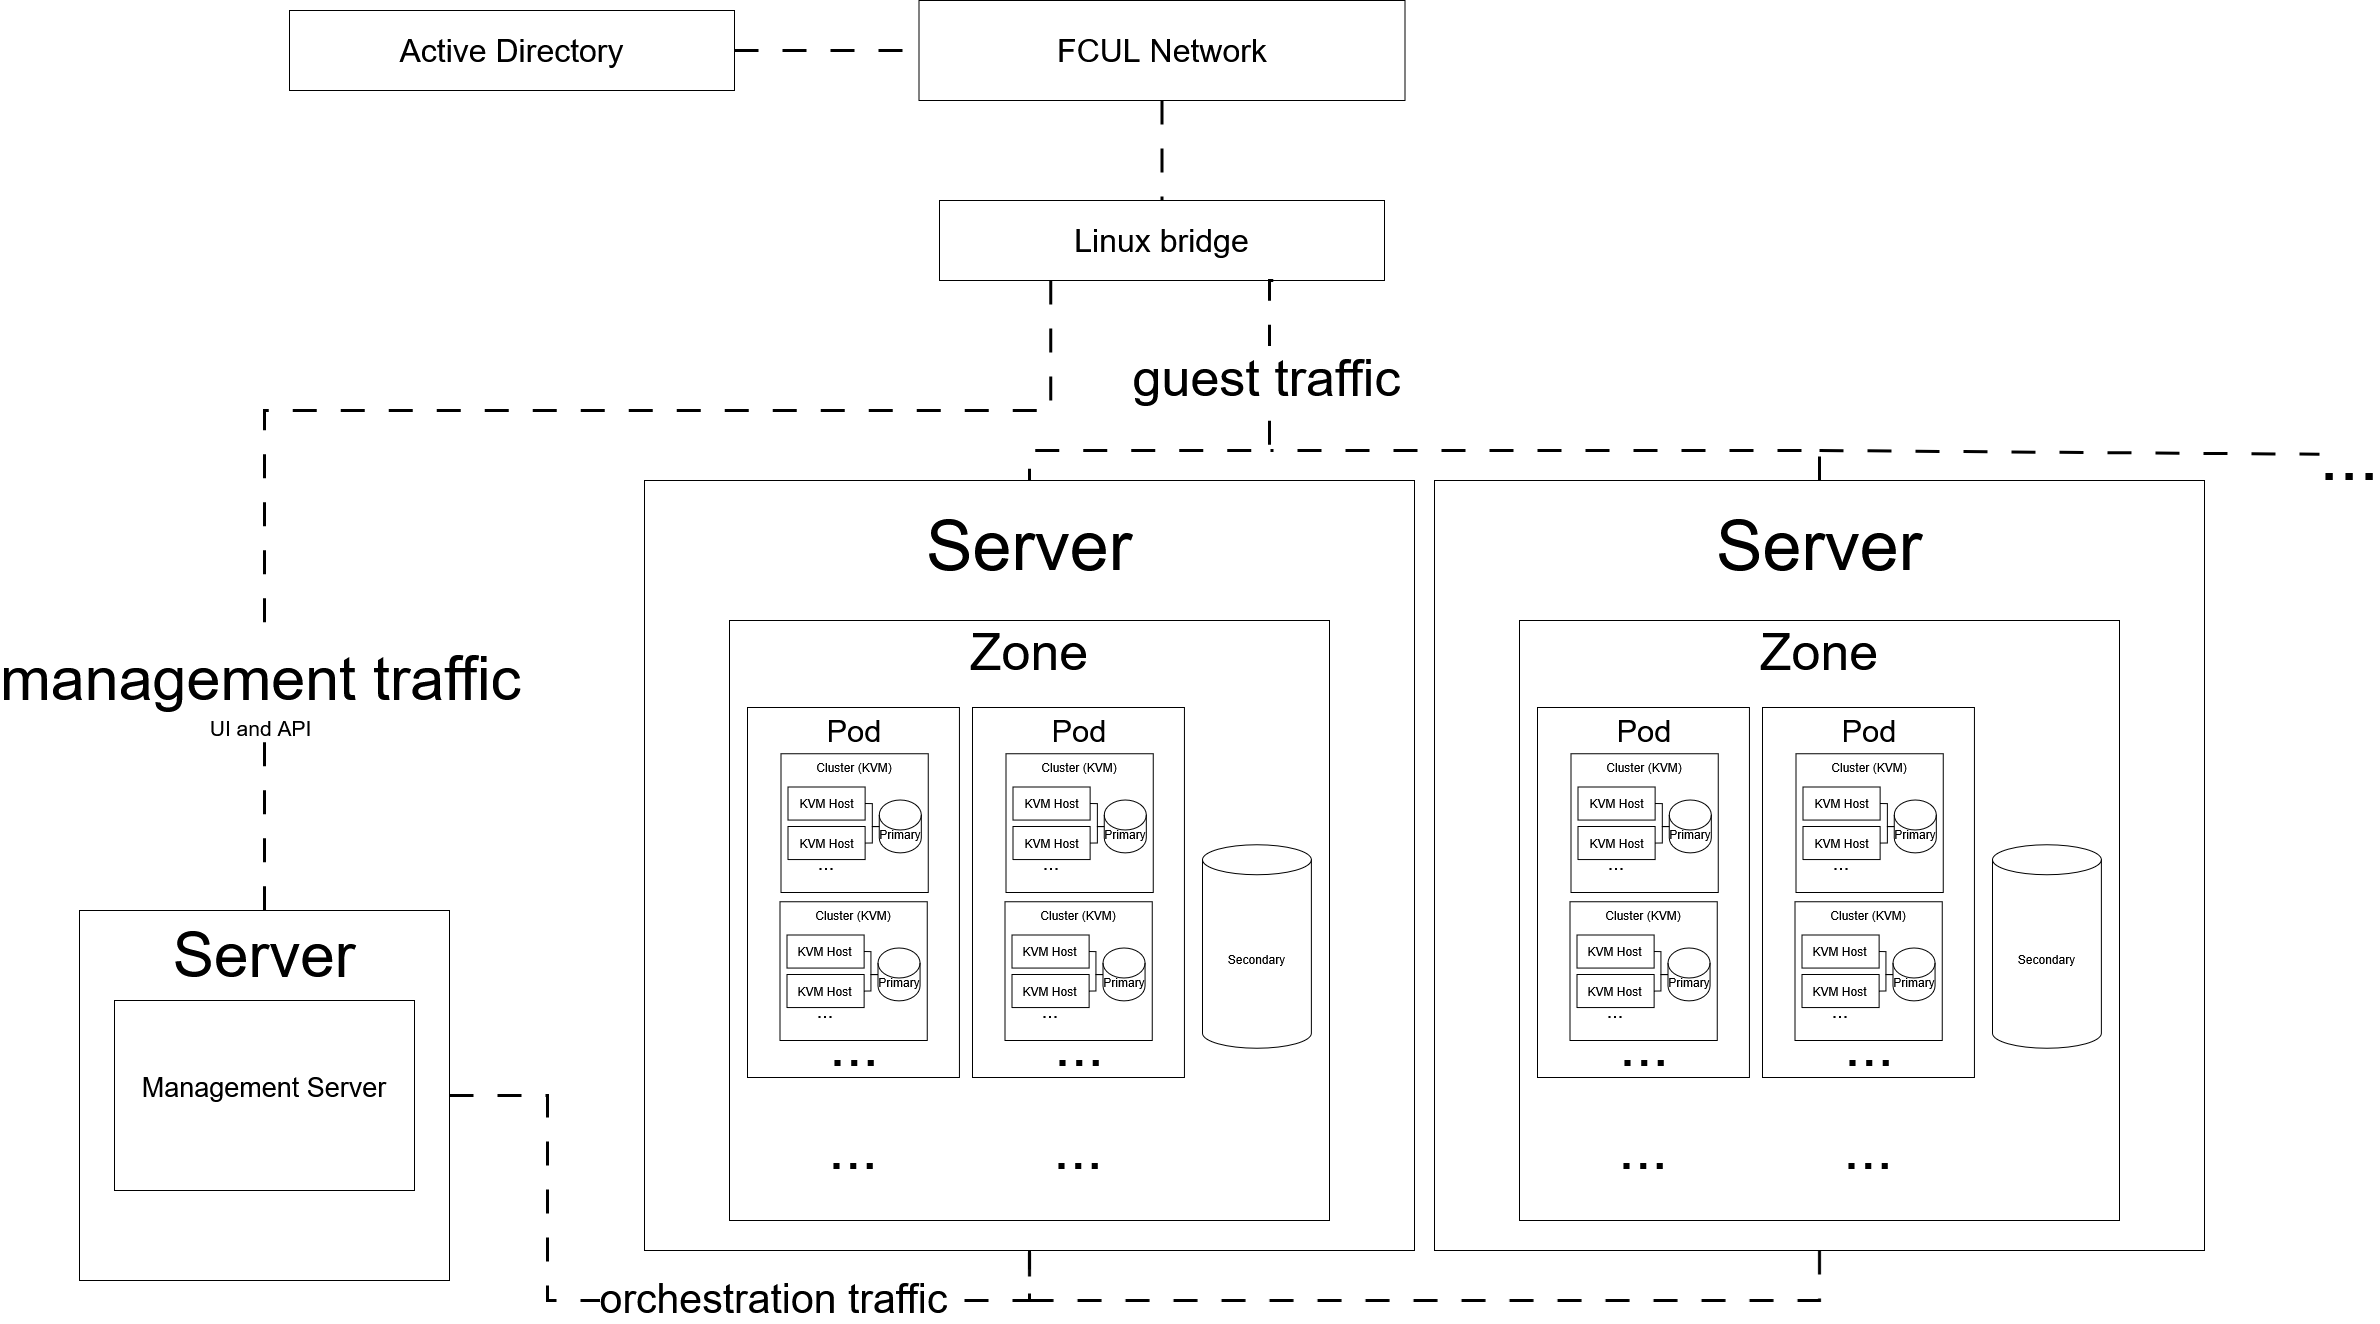
\includegraphics[width=\linewidth]{photos/CloudstackArchitecture.png}
                \caption{Cloudstack Architecture.}
                \label{fig:Cloudstack Architecture}
            \end{figure}
        
        CloudStack is adopted as the core cloud management platform, for the reasons discussed in the previous sections where the platform is analyzed and compared with the alternatives, responsible for orchestrating compute, storage, and networking resources. It provides a centralized control plane through its Management Server, exposing both a web-based interface and API that enables access to CloudStack's services.
        VMs are deployed on host servers running the CloudStack Agent and the KVM hypervisor, which provides native integration with Linux and compatibility with CloudStack through the libvirt interface.\\

        From a storage perspective, the architecture has two types of storage, primary and secondary. The first is created and associated with clusters to host VM disk volumes, and the second is configured at the zone level to support templates, ISO images, and snapshots. These storage components are shared within the cloud environment and are accessed by the hosts under the coordination of the management server.\\

        Similarly, network resources are defined as first-class entities within the cloud platform. Physical and virtual networks are configured during the cloud setup process and are subsequently allocated to virtual machines during deployment. This approach allows networking to be managed consistently as a cloud resource, while preserving compatibility with the existing DI network infrastructure.\\

        Authentication is integrated with the existing Active Directory infrastructure, enabling the usage of the existent institutional accounts and role-based access control. Resource usage is regulated through quotas and service offerings defined at the cloud management level.\\

        The primary objective of the proposed infrastructure is the automated provisioning and management of VM's. Nevertheless, the adopted cloud architecture allows extensibility, making storage and networking cloud resources as well, beyond their role as support mechanisms for virtual machines. In this context, storage pools and virtual networks can be explicitly defined, managed, and reused across deployments, enabling future expansion towards more advanced resource management scenarios without requiring fundamental architectural changes.\\
        
        Overall, this architecture will allow operational simplicity, reuse of infrastructure, and the integration with institutional services already existent. It provides a scalable and maintainable platform for delivering self-service virtualized resources in an academic environment, while remaining aligned with the technical and organizational constraints of DI–FCUL.

    
    \subsection{Methodology and Implementation Strategy}
        The project development follows an incremental and iterative methodology aligned with the project work plan. Although the work is organized into distinct phases, these phases are not strictly sequential and partially overlap in time, allowing certain activities, such as architectural design, deployment, and documentation, to progress in parallel when appropriate. Basically the infrastructure is designed and implemented progressively, allowing each component to be validated before introducing additional complexity.\\

        The implementation begins with the installation and configuration of the selected IaaS platform, Cloudstack, and hypervisor, KVM, on a limited set of servers, establishing a functional POC. This initial setup focuses on core functionalities such as virtual machine provisioning, storage integration, and basic networking. Subsequent steps extend the infrastructure by integrating centralized authentication through the institutional Active Directory and by defining resource management policies, including quotas and service offerings.\\
        
        Throughout the process, the implementation is carried out in close alignment with the existing infrastructure and in collaboration with the SYSADMIN team, ensuring it's compatibility. This phased approach reduces deployment risk, simplifies troubleshooting, and allows early feedback to inform later stages of the project.
    
    \subsection{Validation Strategy}
        The validation of the proposed private cloud infrastructure focuses on demonstrating its functional correctness and suitability for academic use. The validation is conducted through the deployment and evaluation of demonstrative prototypes that reflect realistic usage scenarios.\\

        The validation process includes verifying the platform functions as expected, the successful integration with the Active Directory and the enforcement of access control and resource usage policies. Additional validation criteria include system stability during typical administrative operations and the consistency of resource allocation across different user profiles. System performance is also one of the validation criteria, although the focus of this project is not performance, but a usable simple platform.\\
        
        These validation activities aim to confirm that the defined requirements are satisfied and can be operated reliably, providing a solid foundation for future extensions and broader adoption.

\section{Preliminary Results} \label{sec:results}
    This section presents the preliminary results obtained so far during the development of the proposed private cloud infrastructure. As the project is still ongoing, these results focus on the initial deployment and configuration stages, as well as on early observations derived from the Proof-Of-Concept\footnote{Proof-of-Concept, also known as POC} implementation.

    \subsection{Infrastructure Setup}
        At this stage, a simple and functional POC has been deployed. This initial setup includes the installation and configuration of Apache CloudStack, the integration of KVM, and the configuration of the compute hosts within the cloud environment. A basic cloud structure was defined, including the creation of zones, clusters, and storage components required to support virtual machine provisioning.\\

        The physical server is equipped with two Intel Xeon E5630 processors running at 2.53 GHz, providing a total of 8 Cores and 16 total threads. The system has 8 GB of RAM available and uses a local 500GB hard disk, making this configuration sufficient to support the installation of the cloud management platform, the definition of storage resources, and the provisioning of multiple virtual machines for preliminary validation purposes, although a very limited amount.\\
        
        Primary and secondary storage resources were configured to enable the deployment of virtual machine volumes and templates, allowing fully functional virtual machines to be created and used. Basic networking was also established to ensure connectivity between the management components, hypervisor hosts, and deployed virtual machines.\\
        
        This initial deployment provided valuable insights into potential challenges that may arise during the full-scale implementation and offered hands-on experience with the platform, contributing to a more efficient deployment in subsequent phases.
    
    \subsection{Initial Experiments and Observations}
        Initial experiments revealed several practical challenges inherent to the deployment of a private cloud infrastructure. In particular, issues related to the configuration of Linux bridges were encountered during the initial setup. Although bridge configuration is not specific to Apache CloudStack itself, it is a fundamental component for enabling virtual machine networking in KVM-based environments and proved to be a critical dependency for the correct operation of the platform.\\

        Despite following the official CloudStack documentation and the POC guides, the overall installation and configuration process was more complex than initially anticipated. This complexity stems not only from the cloud management platform but also from the interaction between the hypervisor, networking components, and the existing infrastructure constraints.\\
        
        Another limiting factor during this phase was the availability of a single physical server. While sufficient to validate basic functionality, this setup restricted the ability to test scenarios closer to the intended final deployment, such as communication between multiple compute hosts and the management server over bridged networks. As a result, certain aspects of host-to-management communication and multi-host networking could not yet be fully evaluated.\\
        
        At this stage, no scalability or performance testing has been conducted. These aspects are planned for later phases, once a more representative multi-host environment is available. Nevertheless, the challenges encountered during the initial deployment provided valuable insights into potential configuration pitfalls and reinforced the importance of an incremental deployment strategy, which will facilitate a smoother and more efficient implementation in subsequent phases.

\section{Forthcoming Work and Conclusions} \label{sec:conclusions}
    This section outlines the work planned for the remaining duration of the project and provides a preliminary assessment of the progress achieved so far.

    \subsection{Forthcoming Work}
        The forthcoming work will focus on completing the design, deployment, and validation of the proposed private cloud infrastructure in accordance with the project plan. Following the initial POC deployment, the next planned step will focus on the integration with the institutional Active Directory, enabling centralized auth and role-based access control for different user profiles.\\

        In parallel, the network architecture will be refined to support a multi-host environment, allowing more realistic deployment scenarios to be evaluated. This includes validating communication between compute hosts and the management server through the configured network bridges and ensuring compliance with institutional networking policies. Additional effort will be dedicated to the definition and enforcement of resource management policies, such as quotas and service offerings, in order to regulate resource usage among different user groups.\\
        
        Subsequently, demonstrative prototypes will be prepared to validate the infrastructure under typical academic usage scenarios and to determine whether the platform behaves as expected, is stable, and usable. Throughout these phases, documentation and configuration refinements will be carried out.
    
    \subsection{Project Timeline}
        The remaining work is planned according to an incremental development approach with partial overlap between phases, as reflected in the project Gantt chart, Appendix \ref{appendix:workplan}. While the project is structured into distinct phases, activities such as deployment, integration, validation, and documentation are expected to progress in parallel when appropriate. This approach allows early feedback from preliminary deployments to inform subsequent stages and reduces the risks associated with large, monolithic configuration changes.\\
        
        The project timeline extends until July 2026, with implementation and validation activities concentrated in the first half of 2026, followed by the consolidation of results and the writing of the final dissertation document. This planning ensures a balanced distribution of effort between technical implementation and academic reporting.

    \subsection{Preliminary Self-Assessment}
         At the current stage, the project has established a simple yet functional infrastructure, including the installation and configuration of a suitable operating system, the deployment of the required software components, and an initial CloudStack setup used to explore and test potential future configurations.\\
        
        This phase primarily served to gain hands-on experience with the selected technologies, their configuration workflows, and their operational dependencies. The knowledge obtained during this stage is a solid base for future implementation phases and will allow subsequent development to progress more efficiently and with reduced uncertainty.

    \subsection{Challenges and Difficulties}
        Several challenges were encountered that influenced both the technical implementation and the overall planning. A significant source of complexity arose from the configuration of the underlying infrastructure, particularly regarding network setup and Linux bridge configuration. Although these components are not specific to CloudStack itself, they are essential. bridge-related configuration issues required iterative testing and adjustments, which occupied a non-negligible amount of time during the early deployment phase.\\
        
        Another challenge was the limited availability of servers, as this limited the ability to test scenarios that could resemble the intended final deployment, such as multi-host communication, redundancy, scalability, and high availability. As a result, some validation activities had to be postponed to later phases when additional infrastructure is expected to be available.\\
        
        From a project management perspective, time management also proved to be a challenge. In particular, the time required to review and analyze the relevant literature was underestimated, which temporarily affected the balance between theoretical analysis and hands-on implementation. This experience highlighted the importance of more structured time management in later phases of the project.\\
        
        Despite these difficulties, the challenges encountered contributed positively to the project by deepening the understanding of the platform, its dependencies, and its operational requirements. They also helped identify potential risks early that could delay future progress.

    
    \subsection{Conclusions}
        This report presented the motivation, context, and initial progress of a project aimed at designing and deploying a private IaaS cloud for DI–FCUL. The work carried out so far provides a practical understanding of the architectural and operational aspects involved in deploying a CloudStack-based infrastructure.\\
        
        Although the current implementation is limited, it establishes a solid knowledge foundation for the remaining phases of the project. The challenges encountered during the initial deployment, have shown possible issues that could be found during the future work.\\
        
        The next stages of the project will focus on completing the integration with institutional services, expanding the infrastructure to support multi-host scenarios, and validating the platform under realistic usage conditions. Ultimately, this work aims to deliver a functional, maintainable, and extensible private cloud infrastructure that supports the teaching and research activities of DI–FCUL while reducing administrative overhead through automation and centralized management.

%%%%%%%%%%%%%%%%%%%%%%%%%%%%%%%%%%%%%%%%%%%%%%%%%%%%%%%%%%%%%%%%%%%%%%
%% The next two lines define the bibliography style to be used, and
%% the bibliography file.
\bibliographystyle{ACM-Reference-Format}
\bibliography{sample-base}

\onecolumn
\appendix
\section{Project Work Plan}
\label{appendix:workplan}

This appendix presents the detailed project planning and timeline of the project.
The planning is represented through a Gantt chart, summarizing the main phases,
their expected duration, and the partial overlap between activities, in accordance
with the work plan defined in the project proposal. The bellow Gantt chart could also be found \href{https://github.com/jotanmiguel/ThesisCC25-26/blob/main/documentos/Jo%C3%A3o%20Oliveira%20Thesis%20Gantt%20Chart%2020251214.png}{\textit{here}}

\begin{figure}[H]
    \centering
    \includegraphics[width=\linewidth]{photos/gantt_chart.pdf}
    \caption{Project planning and timeline (Gantt chart).}
    \label{fig:gantt}
\end{figure}

\begin{table}[!ht]
    \raggedleft
    \begin{tabular}{|l|l|l|l|l|}
    \hline
        Task & Start & Finish & Duration & \% Complete \\ \hline
        Thesis & 2025-10-01 & 2026-06-21 & 264 day & 40 \\ \hline
        Phase 1 – Requirements, State of the Art and Report & 2025-10-01 & 2026-01-06 & 98 day & 100 \\ \hline
        Literature review and background study & 2025-10-01 & 2025-11-15 & 46 day & 100 \\ \hline
        Related work consolidation & 2025-11-24 & 2025-12-20 & 27 day & 100 \\ \hline
        EO report writing & 2025-10-11 & 2025-12-30 & 81 day & 100 \\ \hline
        Final revision and submission & 2025-12-24 & 2026-01-06 & 14 day & 100 \\ \hline
        Phase 2 – Access Control System Deployment & 2025-12-04 & 2026-02-23 & 82 day & 15 \\ \hline
        Server Configuration and Solution Installation & 2025-12-04 & 2025-12-22 & 19 day & 75 \\ \hline
        Requirements analysis with DI & 2026-01-03 & 2026-01-15 & 13 day & 0 \\ \hline
        Evaluation of access control solutions & 2026-01-12 & 2026-01-22 & 11 day & 0 \\ \hline
        Deployment and configuration & 2026-01-23 & 2026-02-12 & 21 day & 0 \\ \hline
        Testing and documentation & 2026-02-13 & 2026-02-23 & 11 day & 0 \\ \hline
        Phase 3 – Network Architecture Design and Implementation & 2026-01-03 & 2026-03-13 & 70 day & 0 \\ \hline
        Network requirements analysis & 2026-01-03 & 2026-01-09 & 7 day & 0 \\ \hline
        Network architecture design & 2026-01-10 & 2026-01-23 & 14 day & 0 \\ \hline
        Network implementation & 2026-02-13 & 2026-02-27 & 15 day & 0 \\ \hline
        Network testing and documentation & 2026-02-28 & 2026-03-13 & 14 day & 0 \\ \hline
        Phase 4 – Active Directory Integration & 2026-03-09 & 2026-04-15 & 38 day & 0 \\ \hline
        AD environment analysis and preparation & 2026-03-09 & 2026-03-15 & 7 day & 0 \\ \hline
        Authentication and directory integration & 2026-03-15 & 2026-03-28 & 14 day & 0 \\ \hline
        Role-based access control configuration & 2026-03-24 & 2026-04-08 & 16 day & 0 \\ \hline
        Testing, validation and documentation & 2026-04-04 & 2026-04-15 & 12 day & 0 \\ \hline
        Phase 5 – Prototypes and Validation & 2026-04-15 & 2026-05-15 & 31 day & 0 \\ \hline
        Definition of validation scenarios & 2026-04-15 & 2026-04-21 & 7 day & 0 \\ \hline
        Prototype deployment & 2026-04-20 & 2026-05-03 & 14 day & 0 \\ \hline
        Functional validation & 2026-04-29 & 2026-05-12 & 14 day & 0 \\ \hline
        Documentation of results and limitations & 2026-04-22 & 2026-05-15 & 24 day & 0 \\ \hline
        Phase 6 – Final Thesis Writing & 2026-05-06 & 2026-06-21 & 47 day & 0 \\ \hline
        Writing of implementation chapters & 2026-05-06 & 2026-05-19 & 14 day & 0 \\ \hline
        Writing of results and validation chapters & 2026-05-20 & 2026-06-02 & 14 day & 0 \\ \hline
        Discussion and conclusions & 2026-06-03 & 2026-06-09 & 7 day & 0 \\ \hline
        Final revision and submission & 2026-06-10 & 2026-06-21 & 12 day & 0 \\ \hline
    \end{tabular}
\end{table}

\end{document}
